\section{SequenceViewer}\label{sec:sequenceviewer}
The GIRAF-project contains three applications which share a common feature regarding sequences of pictograms. The three applications are Sekvens, Livshistorier, and PiktoOplæser. During sprint 2, the groups held a meeting regarding a common need for storing sequences in the database. During this meeting, a new project was established, namely Sequenceviewer. The Seqeuenceviewer was decided to be a front-end application, which the three other applications should call whenever they want to display a sequence to a child. This new application should ensure a common interface whenever the children interact with the system. The sequences of pictograms will be displayed in the same way, whichever application they previously used to make a sequence of pictograms.

The purpose of Sequenceviewer is to act as a service to the three other applications. It is not suppose to be apparent to the guardians or the children, that they actually enter the Sequenceviewer application. The position of Sequenceviewer in the GIRAF multiproject is shown in figure \ref{fig:sequenceviewer}.

\begin{figure}[H]
	\centering
	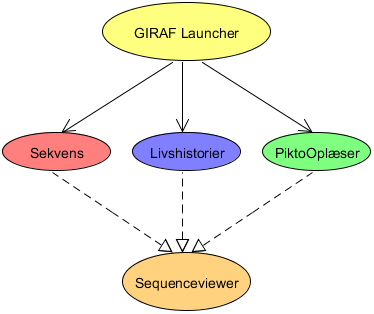
\includegraphics[scale=0.8]{Pics/sequenceviewer}
	\caption{The position of Sequenceviewer in the GIRAF multiproject.}
	\label{fig:sequenceviewer}
\end{figure}

The stippled lines between the three applications and Sequenceviewer, represent the fact that it should not be apparent to the users that they enter Sequenceviewer.

